% Copyright 2004 by Till Tantau <tantau@users.sourceforge.net>.
%
% In principle, this file can be redistributed and/or modified under
% the terms of the GNU Public License, version 2.
%
% However, this file is supposed to be a template to be modified
% for your own needs. For this reason, if you use this file as a
% template and not specifically distribute it as part of a another
% package/program, I grant the extra permission to freely copy and
% modify this file as you see fit and even to delete this copyright
% notice. 

\documentclass{beamer}

% There are many different themes available for Beamer. A comprehensive
% list with examples is given here:
% http://deic.uab.es/~iblanes/beamer_gallery/index_by_theme.html
% You can uncomment the themes below if you would like to use a different
% one:
%\usetheme{AnnArbor}
%\usetheme{Antibes}
%\usetheme{Bergen}
%\usetheme{Berkeley}
%\usetheme{Berlin}
%\usetheme{Boadilla}
%\usetheme{boxes}
%\usetheme{CambridgeUS}
%\usetheme{Copenhagen}
%\usetheme{Darmstadt}
%\usetheme{default}
%\usetheme{Frankfurt}
%\usetheme{Goettingen}
%\usetheme{Hannover}
%\usetheme{Ilmenau}
%\usetheme{JuanLesPins}
%\usetheme{Luebeck}
\usetheme{Madrid}
%\usetheme{Malmoe}
%\usetheme{Marburg}
%\usetheme{Montpellier}
%\usetheme{PaloAlto}
%\usetheme{Pittsburgh}
%\usetheme{Rochester}
%\usetheme{Singapore}
%\usetheme{Szeged}
%\usetheme{Warsaw}
% \usepackage{graphicx}
% \graphicspath{ {/home/ajay/Pictures/} }

\title{Case Study 1}

% A subtitle is optional and this may be deleted
\subtitle{Image filtering using diffusion models}

\author{Alfred Ajay Aureate R\inst{1}}
% - Give the names in the same order as the appear in the paper.
% - Use the \inst{?} command only if the authors have different
%   affiliation.

\institute[IITM] % (optional, but mostly needed)
{
  \inst{1}%
  EE10B052\\
  Department of Electrical Engineering\\
  Indian Institute of Technology Madras}
% - Use the \inst command only if there are several affiliations.
% - Keep it simple, no one is interested in your street address.

\date{MA5710, Dec 2014}
% - Either use conference name or its abbreviation.
% - Not really informative to the audience, more for people (including
%   yourself) who are reading the slides online

\subject{Mathematics}
% This is only inserted into the PDF information catalog. Can be left
% out. 

% If you have a file called "university-logo-filename.xxx", where xxx
% is a graphic format that can be processed by latex or pdflatex,
% resp., then you can add a logo as follows:

% \pgfdeclareimage[height=0.5cm]{university-logo}{university-logo-filename}
% \logo{\pgfuseimage{university-logo}}

% Delete this, if you do not want the table of contents to pop up at
% the beginning of each subsection:
\AtBeginSubsection[]
{
  \begin{frame}<beamer>{Outline}
    \tableofcontents[currentsection,currentsubsection]
  \end{frame}
}

% Let's get started
\begin{document}

\begin{frame}
  \titlepage
\end{frame}

\begin{frame}{Outline}
  \tableofcontents
  % You might wish to add the option [pausesections]
\end{frame}

% Section and subsections will appear in the presentation overview
% and table of contents.
\section{Models Description}

\begin{frame}{Diffusion models description}{}
  \begin{itemize}
  \item {
    The intensity of each pixel of an image is collectively assumed as a matrix $U$.
    \pause
  }
  \item {
    Now, when noise is added to this image, it creates glitches and discontinuities at random pixels. So, by using a diffusion model, we try to smooth-en those discontinuities.
    \pause
  }
  \item {
    Some invariant properties for image:
    \begin{itemize}
    \item {Clean and translate, and translate and clean should give same output}
    \item {Clean and rotate, and rotate and clean should give same output}
    \item {Clean and zoom, and zoom and clean should give same output}
    \item {When a constant is added, we should be able to remove it}
    \end{itemize}
    \pause
  }
  \item {
    $U_{t}=\nabla.\left(D\left(U\right)\nabla U\right)$; $U\left(x,y,0\right)=U_{0}\left(x,y\right)$;
$\frac{\partial U}{\partial n}=0$ on $\partial\Omega$.
  }
  \end{itemize}
\end{frame}

\subsection{Linear Diffusion model}

\begin{frame}{Linear diffusion model}{}
  \begin{itemize}
  \item {
    Here $D\left(U\right)=I$.
    \pause
  }
  \item {
    So, the model becomes $U_{t}=\nabla.\left(I\nabla U\right)$; $U\left(x,y,0\right)=U_{0}\left(x,y\right)$;
$\frac{\partial U}{\partial n}=0$ on $\partial\Omega$.
    \pause
  }
  \item {
    $U\left(x,y,0\right)=U_{0}\left(x,y\right)$. It is the noise-added image before filtering
    \pause
  }
  \item {
    Here, we use Neumann boundary conditions for images
    \pause
  }
  \item {
    It can be proved that the solution for the above equation could be given by: \[
U\left(x,y,t\right)=\begin{cases}
\begin{array}{c}
U_{0}\left(x,y\right)\\
(k_{\sqrt{2t}}*U_{0})\left(x,y\right)
\end{array} & \begin{array}{c}
\left(t=0\right)\\
\left(t>0\right)
\end{array}\end{cases}
\] where $k_{\sqrt{2t}}\left(x,y\right)$ is the gaussian kernel with variance $\sigma=\sqrt{2t}$
  }
  \end{itemize}
\end{frame}

\begin{frame}{Linear diffusion model}
    \begin{itemize}
    \item {}
    \end{itemize}
\end{frame}

\subsection{Non-linear Perona-Malik diffusion model}

% You can reveal the parts of a slide one at a time
% with the \pause command:
\begin{frame}{Perona-Malik diffusion model}
  \begin{itemize}
  \item {
    This is part of the non-linear scalar diffusion model. So, $D\left(U\right)=c\left(\Vert\nabla U\Vert\right)I$, where $c\left(\Vert\nabla U\Vert\right)=\frac{1}{1+\frac{\Vert\nabla U\Vert^{2}}{\lambda^{2}}}$.
    \pause % The slide will pause after showing the first item
  }
  \item {   
    So, the model becomes $U_{t}=\nabla.\left(c\left(\Vert\nabla U\Vert\right)I\nabla U\right)$;
$U\left(x,y,0\right)=U_{0}\left(x,y\right)$; $\frac{\partial U}{\partial n}=0$
on $\partial\Omega$; where $c\left(\Vert\nabla U\Vert\right)=\frac{1}{1+\frac{\Vert\nabla U\Vert^{2}}{\lambda^{2}}}$ 
    \pause
  }
  % You can also specify when the content should appear
  % by using <n->:
  \item<3-> {
    $U\left(x,y,0\right)=U_{0}\left(x,y\right)$. It is the noise-added image before filtering
    \pause
  }
  \item<4-> {
    Here, we use Neumann boundary conditions for images
    \pause
  }
  % or you can use the \uncover command to reveal general
  % content (not just \items):
  \item<5-> {
    Catte extended this model, which is now called the PMC diffusion model. \uncover<6->{Basically, here PM model is applied to $U_{\sigma}$, which is the solution of the linear diffusion model, rather than using just $U$ for the PM model. So, in PMC model, $U_{t}=\nabla.\left(c\left(\Vert\nabla U_{\sigma}\Vert\right)I\nabla U_{\sigma}\right)$.  $U_{\sigma}$ is the solution got from the linear diffusion model, where $U_{0}$ is convolved with a gaussian kernel of variance $\sigma$.}
  }
  \end{itemize}
\end{frame}


\subsection{Non-linear Edge enhancing diffusion model}

% You can reveal the parts of a slide one at a time
% with the \pause command:
\begin{frame}{Edge enhancing diffusion model}
  \begin{itemize}
  \item {
    This is part of the non-linear tensor diffusion model. So, $D=\left[\begin{array}{cc}
a & b\\
c & d
\end{array}\right]$.
    \pause % The slide will pause after showing the first item
  }
  \item {   
    Now, for the edge-enhancing diffusion model, the diffusion tensor is given by: 
\[
D=R^{T}\left(\begin{array}{cc}
c_{1} & 0\\
0 & c_{2}
\end{array}\right)R
\]
 where $R$ is the rotation matrix describing the local coordinate system aligned with the gradient vector observed at scale $u$.
    \pause
  }
  % You can also specify when the content should appear
  % by using <n->:
  \item<3-> {
    \[
R=\frac{1}{\sqrt{\left(L_{x}^{u}\right)^{2}+\left(L_{y}^{u}\right)^{2}}}\left(\begin{array}{cc}
L_{x}^{u} & -L_{y}^{u}\\
L_{y}^{u} & L_{x}^{u}
\end{array}\right)
\]
where $L^{u}$ denotes the image observed at scale $u$.
  }
  \end{itemize}
\end{frame}

\begin{frame}{Edge enhancing diffusion model}
  \begin{itemize}
  \item{$c_{1}$ is the conductivity in the direction of the gradient (observed at scale $u$) and the $c_{2}$ is the conductivity along the isophote. Inorder to compare edge-enhancing diffusion with scalar difusion (Perona and Malik type) we set the diffusion along the edge to be equal to the isotropic diffusion in the Perona malik diffusion discussed earlier and set the conductivity across the edge to be one fifth of the conductivity along the edge. \[c_{2}\left(L_{w}^{u}\right)=\frac{1}{1+\frac{\left(L_{w}^{u}\right)^{2}}{\lambda^{2}}}\]
\[c_{1}\left(L_{w}^{u}\right)=\frac{1}{5}c_{2}\left(L_{w}^{u}\right)\] Here, $L_{w}^{u}=\sqrt{\left(L_{x}^{u}\right)^{2}+\left(L_{y}^{u}\right)^{2}}$ is the gradient norm.}
  \end{itemize}
\end{frame}

\section{Implementation of models}

\subsection{Linear diffusion model}

\begin{frame}{Linear diffusion model}
    \begin{itemize}
    \item {The following line implements linear diffusion model in the code: \[g=gD(g,0.4,0,0)\]}
    \end{itemize}
\begin{figure}
\caption{Original noisy image vs Linear Diffused image}
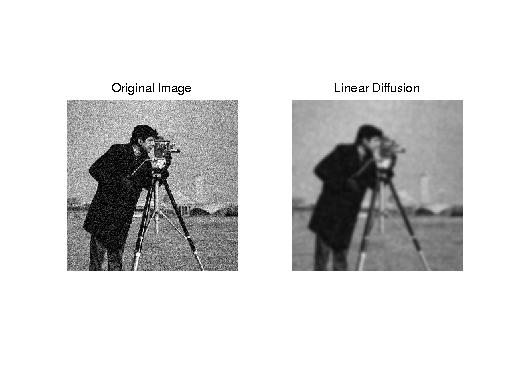
\includegraphics[scale=0.5]{ld.jpg}
\end{figure}
\end{frame}

\subsection{Perona Malik model}

\begin{frame}{Perona Malik model}
    \begin{itemize}
    \item {The following line implements linear diffusion model in the code: \[g=gD(g,0.4,0,0)\]}
    \end{itemize}
\begin{figure}
\caption{Original noisy image vs Linear Diffused image}
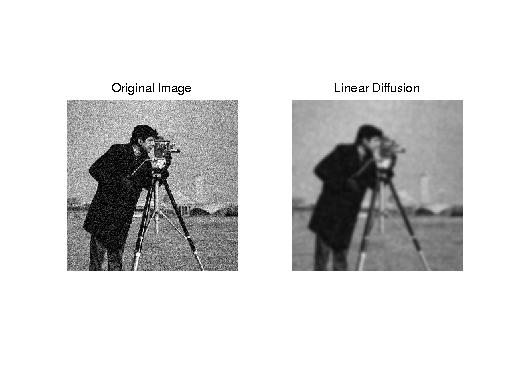
\includegraphics[scale=0.5]{ld.jpg}
\end{figure}
\end{frame}

% Placing a * after \section means it will not show in the
% outline or table of contents.
\section*{Summary}

\begin{frame}{Summary}
  \begin{itemize}
  \item
    The \alert{first main message} of your talk in one or two lines.
  \item
    The \alert{second main message} of your talk in one or two lines.
  \item
    Perhaps a \alert{third message}, but not more than that.
  \end{itemize}
  
  \begin{itemize}
  \item
    Outlook
    \begin{itemize}
    \item
      Something you haven't solved.
    \item
      Something else you haven't solved.
    \end{itemize}
  \end{itemize}
\end{frame}



% All of the following is optional and typically not needed. 
\appendix
\section<presentation>*{\appendixname}
\subsection<presentation>*{For Further Reading}

\begin{frame}[allowframebreaks]
  \frametitle<presentation>{For Further Reading}
    
  \begin{thebibliography}{10}
    
  \beamertemplatebookbibitems
  % Start with overview books.

  \bibitem{Author1990}
    A.~Author.
    \newblock {\em Handbook of Everything}.
    \newblock Some Press, 1990.
 
    
  \beamertemplatearticlebibitems
  % Followed by interesting articles. Keep the list short. 

  \bibitem{Someone2000}
    S.~Someone.
    \newblock On this and that.
    \newblock {\em Journal of This and That}, 2(1):50--100,
    2000.
  \end{thebibliography}
\end{frame}

\end{document}



